\section{Logistic regression}
\label{sec:logistic_regression}

The logistic regression model predicts the probability that an observation
belongs to a class. Unlike the Gaussian discriminant model of
Section~\ref{sec:discriminant_analysis}, which specifies the distribution of
$\vb{X}$ \emph{within} each class and then inverts it with Bayes' theorem, here
the posterior probability itself is modelled directly as a function of the
predictors.

\subsection{The logistic function}
\label{subsec:logistic_function}

\begin{definition}[Logistic function]
  \label{def:logistic_function}
  The \textbf{logistic function} is
  \begin{equation}
    \label{eq:logistic}
    p=\si(z)=\frac{1}{1+e^{-z}},
    \qquad z\in\R .
  \end{equation}
\end{definition}

It is strictly increasing, satisfies $\si(z)\to 0$ as $z\to-\infty$ and
$\si(z)\to 1$ as $z\to+\infty$, and $\si(0)=\tfrac12$; hence it is a bijection
\begin{equation}
  \label{eq:logistic_bijection}
  \R\longleftrightarrow(0,1),
\end{equation}
which is precisely what is needed to turn an unbounded linear predictor into a
probability.

\begin{figure}[H]
  \centering
  \begin{tikzpicture}[scale=0.85]
    \draw[dashed,gray] (-3.3,1.7) -- (3.3,1.7);
    \draw[->] (-3.3,0) -- (3.6,0) node[right] {\footnotesize $z$};
    \draw[->] (0,-0.25) -- (0,2.1) node[above] {\footnotesize $p$};
    \node[above left,inner sep=1pt] at (0,1.7) {\footnotesize $1$};
    \node[below left,inner sep=1pt] at (0,0) {\footnotesize $0$};
    \node[below] at (-3,0) {\footnotesize $-10$};
    \node[below] at (3,0) {\footnotesize $10$};
    \draw[thick,domain=-3.2:3.2,samples=150,smooth]
      plot (\x,{1.7/(1+exp(-2.2*\x))});
    \node[right] at (0.9,1.15) {\footnotesize $\dfrac{1}{1+e^{-z}}$};
  \end{tikzpicture}
  \caption{The logistic curve maps $\R$ onto $(0,1)$.}
  \label{fig:logistic_curve}
\end{figure}

\subsection{The logit transformation}
\label{subsec:logit}

Solving \eqref{eq:logistic} for $z$ in terms of $p$ gives
\begin{equation}
  \label{eq:logit_derivation}
  \begin{aligned}
    p=\frac{1}{1+e^{-z}}
      &\imp p\qty{1+e^{-z}}=1
       \imp 1+e^{-z}=\frac{1}{p}\\
      &\imp e^{-z}=\frac{1}{p}-1=\frac{1-p}{p}\\
      &\imp -z=\log\qty{\frac{1-p}{p}}\\
      &\imp z=\log\qty{\frac{p}{1-p}} .
  \end{aligned}
\end{equation}

\begin{definition}[Logit function]
  \label{def:logit}
  The inverse of \eqref{eq:logistic} is the \textbf{logit function}
  \begin{equation}
    \label{eq:logit}
    z=\operatorname{logit}(p)=\log\qty{\frac{p}{1-p}},
    \qquad p\in(0,1),
  \end{equation}
  which transforms probabilities into real values.
\end{definition}

The argument of \eqref{eq:logit} is itself worth naming.

\begin{definition}[Odds]
  \label{def:odds}
  The \textbf{odds} (\emph{oportunidad a momio}) associated with a probability
  $p$ is
  \begin{equation}
    \label{eq:odds}
    \frac{p}{1-p}\in(0,\infty),
  \end{equation}
  the ratio between the probability of the event and that of its complement.
\end{definition}

So the logit is the logarithm of the odds, and \eqref{eq:logistic} and
\eqref{eq:logit} are inverse to each other.

\subsection{The model}
\label{subsec:logistic_model}

Suppose the response variable $Y_0$ takes the values $0$ and $1$, and that a
vector of predictors
\begin{equation}
  \label{eq:predictor_vector}
  \vb{X}_0^\tp=(X_{01},X_{02},\dots,X_{0p})
\end{equation}
is observed. Write
\begin{equation}
  \label{eq:p_definition}
  p=\mathbb{P}\qty{Y_0=1\such\vb{X}_0=\vb{x}_0},
\end{equation}
so that, conditionally on the predictors,
\begin{equation}
  \label{eq:bernoulli}
  Y_0\such\qty{\vb{X}_0=\vb{x}_0}\sim\text{Bernoulli}(p).
\end{equation}

\begin{definition}[Logistic regression model]
  \label{def:logistic_regression}
  The \textbf{logistic regression model} assumes that the logit of $p$ is an
  affine function of the predictors,
  \begin{equation}
    \label{eq:logistic_model}
    z=\log\qty{\frac{p}{1-p}}
      =\be_0+\be_1x_{01}+\dots+\be_px_{0p}.
  \end{equation}
\end{definition}

Inverting \eqref{eq:logistic_model} with \eqref{eq:logistic} recovers the
probability,
\begin{equation}
  \label{eq:logistic_probability}
  p=\si(z)=\frac{1}{1+e^{-\left(\be_0+\be_1x_{01}+\dots+\be_px_{0p}\right)}},
\end{equation}
and exponentiating \eqref{eq:logistic_model} gives the odds
\begin{equation}
  \label{eq:odds_model}
  \frac{p}{1-p}=e^{\left(\be_0+\be_1x_{01}+\dots+\be_px_{0p}\right)}.
\end{equation}

\begin{remark}
  Equation \eqref{eq:odds_model} is what makes the coefficients interpretable.
  Increasing $x_{0j}$ by one unit, with all other predictors held fixed,
  multiplies the odds by $e^{\be_j}$; the effect is additive on the log-odds
  scale and multiplicative on the odds scale, but \emph{not} linear on the
  probability scale.
\end{remark}

\subsection{The logistic classifier}
\label{subsec:logistic_classifier}

The model returns a probability, not a class. To obtain a classification
function in the sense of Section~\ref{sec:discriminant_analysis} one fixes a
\textbf{threshold} $\tau\in(0,1)$ and assigns
\begin{equation}
  \label{eq:logistic_rule}
  g(\vb{x}_0)=
  \begin{cases}
    1, & p\ge\tau,\\
    0, & p<\tau .
  \end{cases}
\end{equation}

The \textbf{decision boundary} is the set where the two classes are declared
equally plausible, that is, where $p=\tau$. Applying the logit to both sides and
using \eqref{eq:logistic_model},
\begin{equation}
  \label{eq:decision_boundary}
  \log\qty{\frac{\tau}{1-\tau}}
    =\be_0+\be_1x_{01}+\dots+\be_px_{0p}.
\end{equation}
In particular, for the symmetric threshold $\tau=\tfrac12$ the left-hand side
vanishes and the boundary is
\begin{equation}
  \label{eq:decision_boundary_half}
  0=\be_0+\be_1x_{01}+\dots+\be_px_{0p}.
\end{equation}

\begin{remark}
  Equation \eqref{eq:decision_boundary} is affine in $\vb{x}_0$, so the boundary
  is a hyperplane, exactly as in \eqref{eq:delta_ij}: changing $\tau$ only
  shifts the intercept, never the orientation. Logistic regression and LDA
  therefore produce boundaries of the same shape; what differs is how the
  coefficients are obtained --- LDA estimates $\mub_i$ and $\Si$ and derives
  them, whereas logistic regression fits them directly.
\end{remark}

\begin{figure}[H]
  \centering
  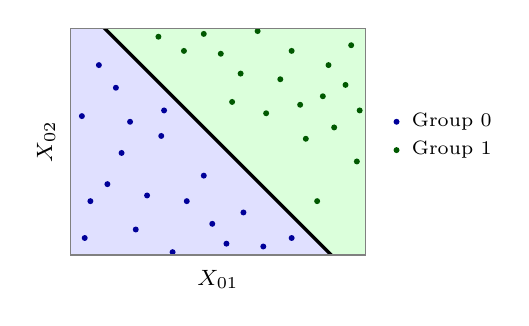
\begin{tikzpicture}[scale=0.72]
    \begin{scope}
      \clip (-2.6,-2.0) rectangle (2.6,2.0);
      \fill[blue!12]  (-2.6,-2.0) -- (2.6,-2.0) -- (-2.6,2.6) -- cycle;
      \fill[green!14!white] (2.6,2.0) -- (2.6,-2.6) -- (-2.6,2.6) -- cycle;
      \foreach \p in {(-2.35,-1.70),(-1.95,-0.75),(-2.40,0.45),(-1.45,-1.55),
                      (-1.00,0.10),(-1.80,0.95),(-0.55,-1.05),(-1.70,-0.20),
                      (0.15,-1.80),(-0.80,-1.95),(0.80,-1.85),(-2.25,-1.05),
                      (-0.25,-0.60),(-1.25,-0.95),(0.45,-1.25),(-2.10,1.35),
                      (-1.55,0.35),(-0.10,-1.45),(1.30,-1.70),(-0.95,0.55)}
        \fill[blue!60!black] \p circle (1.5pt);
      \foreach \p in {(2.35,1.70),(1.85,0.80),(2.45,-0.35),(1.30,1.60),
                      (0.85,0.50),(1.75,-1.05),(0.40,1.20),(1.55,0.05),
                      (-0.25,1.90),(0.70,1.95),(-1.05,1.85),(2.25,1.00),
                      (0.25,0.70),(1.10,1.10),(2.05,0.25),(0.05,1.55),
                      (1.95,1.35),(2.50,0.55),(-0.60,1.60),(1.45,0.65)}
        \fill[green!35!black] \p circle (1.5pt);
      \draw[very thick] (-2.9,2.9) -- (2.9,-2.9);
    \end{scope}
    \draw[gray] (-2.6,-2.0) rectangle (2.6,2.0);
    \node[below] at (0,-2.1) {\footnotesize $X_{01}$};
    \node[left,rotate=90,anchor=south] at (-2.7,0) {\footnotesize $X_{02}$};
    \fill[blue!60!black] (3.15,0.35) circle (1.5pt);
      \node[right,font=\scriptsize] at (3.25,0.35) {Group $0$};
    \fill[green!35!black] (3.15,-0.15) circle (1.5pt);
      \node[right,font=\scriptsize] at (3.25,-0.15) {Group $1$};
  \end{tikzpicture}
  \caption{Example of the logistic classifier: the decision boundary
    \eqref{eq:decision_boundary_half} separates the two groups by a straight
    line in the plane of the predictors.}
  \label{fig:logistic_classifier}
\end{figure}

\subsection{Estimating the coefficients}
\label{subsec:logistic_estimation}

The coefficients $\be^\tp=(\be_0,\be_1,\dots,\be_p)$ are unknown and must be
estimated from a labelled sample $\set{(\vb{x}_n,y_n)}_{n=1}^{m}$ with
$y_n\in\set{0,1}$. Write
\begin{equation}
  \label{eq:pn}
  p_n=\si\qty{\be_0+\sum_{j=1}^{p}\be_j x_{nj}}
\end{equation}
for the probability the model assigns to the $n$-th observation. Because the
observations are independent Bernoulli variables \eqref{eq:bernoulli}, the
likelihood is
\begin{equation}
  \label{eq:likelihood}
  L(\be)=\prod_{n=1}^{m}p_n^{\,y_n}\qty{1-p_n}^{1-y_n},
\end{equation}
and its logarithm, the \textbf{log-likelihood}, is
\begin{equation}
  \label{eq:loglikelihood}
  \ell(\be)=\sum_{n=1}^{m}
    \sqty{y_n\log p_n+(1-y_n)\log\qty{1-p_n}} .
\end{equation}

\begin{definition}[Maximum likelihood estimator]
  \label{def:mle_logistic}
  The estimator $\hat{\be}$ is the maximiser of \eqref{eq:loglikelihood},
  \begin{equation}
    \label{eq:mle_logistic}
    \hat{\be}=\arg\max_{\be}\ \ell(\be).
  \end{equation}
\end{definition}

Collecting the predictors in the $m\times(p+1)$ design matrix $\mat{X}$ whose
first column is a column of ones, and writing $\vb{p}=(p_1,\dots,p_m)^\tp$, the
score equations obtained from \eqref{eq:loglikelihood} are
\begin{equation}
  \label{eq:score}
  \pdv{\ell}{\be}=\mat{X}^\tp\qty{\vb{y}-\vb{p}}=\vb{0}.
\end{equation}

\begin{remark}
  System \eqref{eq:score} is nonlinear in $\be$, because $\vb{p}$ depends on
  $\be$ through the logistic function, and admits no closed-form solution ---
  in contrast with ordinary least squares. It is solved numerically by
  Newton--Raphson, which in this setting takes the form of
  \emph{iteratively reweighted least squares},
  \begin{equation}
    \label{eq:irls}
    \be^{(t+1)}=\be^{(t)}
      +\qty{\mat{X}^\tp\mat{W}\mat{X}}\inv\mat{X}^\tp\qty{\vb{y}-\vb{p}},
  \end{equation}
  with $\mat{W}=\diag\set{p_n(1-p_n)}$. Since $\ell$ is concave, the maximum is
  unique whenever the classes are not perfectly separable.
\end{remark}

\begin{remark}
  In \textsf{R} the model is fitted with
  \texttt{glm(y \textasciitilde\ x, family = binomial)}.
\end{remark}

\subsection{Adequacy of the model}
\label{subsec:logistic_adequacy}

To decide whether a subset of the predictors can be dropped one compares a
\textbf{reduced} model, with $q$ of the coefficients set to zero, against the
\textbf{full} model, by means of the \textbf{likelihood ratio test}. The
hypotheses are
\begin{equation}
  \label{eq:lrt_hypotheses}
  \begin{aligned}
    H_0&:\ \be_{j_1}=\dots=\be_{j_q}=0,\\
    H_1&:\ \text{at least one of them is nonzero,}
  \end{aligned}
\end{equation}
and the statistic is
\begin{equation}
  \label{eq:lrt}
  \La=-2\sqty{\ell\qty{\hat{\be}_{\text{red}}}
              -\ell\qty{\hat{\be}_{\text{full}}}},
\end{equation}
which under $H_0$ is asymptotically distributed as $\chi^2_q$. Large values of
\eqref{eq:lrt} indicate that the reduced model fits significantly worse, so
$H_0$ is rejected and the predictors are kept.

\begin{remark}
  Taking as reduced model the one with only the intercept
  ($\be_1=\dots=\be_p=0$) turns \eqref{eq:lrt} into a global test of the whole
  regression, the analogue of the overall $F$ test in linear regression.
\end{remark}

\selectlanguage{spanish}
\subsection{Resumen del proceso}
\label{subsec:resumen_logistica}

La regresi\'on log\'istica predice la probabilidad de que una observaci\'on
pertenezca a una clase, modelando directamente
$p=\mathbb{P}(Y_0=1\such\vb{X}_0=\vb{x}_0)$ en lugar de la distribuci\'on de las
predictoras dentro de cada grupo.

\begin{enumerate}
  \item La funci\'on log\'istica $\si(z)=1/(1+e^{-z})$ transforma la recta real
        en el intervalo $(0,1)$, de modo que su salida puede leerse como una
        probabilidad.
  \item Su inversa es la funci\'on \textbf{logit},
        $z=\log\qty{p/(1-p)}$, que transforma probabilidades en valores reales;
        el cociente $p/(1-p)$ es la \emph{oportunidad a momio} (\emph{odds}).
  \item El modelo supone $Y_0\such(\vb{X}_0=\vb{x}_0)\sim$ Bernoulli$(p)$ con
        $\operatorname{logit}(p)=\be_0+\be_1x_{01}+\dots+\be_px_{0p}$; al
        despejar, $p=\si(z)$ y los momios quedan como en
        \eqref{eq:odds_model}. Por eso $e^{\be_j}$ es el factor por el que se
        multiplican los momios al aumentar $x_{0j}$ en una unidad.
  \item Para clasificar se fija un umbral $\tau\in(0,1)$; la frontera de
        decisi\'on est\'a dada por
        $\log\qty{\tau/(1-\tau)}=\be_0+\dots+\be_px_{0p}$, que es un hiperplano.
        Con $\tau=1/2$ la frontera es $0=\be_0+\dots+\be_px_{0p}$.
  \item Los coeficientes se estiman por \textbf{m\'axima verosimilitud}; las
        ecuaciones de score $\mat{X}^\tp(\vb{y}-\vb{p})=\vb{0}$ no tienen
        soluci\'on cerrada y se resuelven de forma iterativa.
  \item La adecuaci\'on del modelo se eval\'ua con la \textbf{prueba de raz\'on
        de verosimilitudes}, comparando el modelo completo contra uno reducido
        mediante el estad\'istico \eqref{eq:lrt}, que bajo $H_0$ es
        asint\'oticamente $\chi^2_q$.
\end{enumerate}
\selectlanguage{english}
